\documentclass{article}
\usepackage[utf8]{inputenc}
\usepackage{amsmath}
\usepackage{amssymb}
\usepackage{biblatex}
\usepackage{listings,comment}
\usepackage{verbatim}
\usepackage{siunitx}
\usepackage{booktabs}
\usepackage{tablefootnote}
\newcommand{\tabitem}{~~\llap{\textbullet}~~}
\usepackage[dvipsnames]{xcolor}
\usepackage{tikz}
\usetikzlibrary{arrows.meta}
\usetikzlibrary{arrows}
\usetikzlibrary{shapes.geometric}
\usepackage{tcolorbox}

\addbibresource{mlp_smt_closed.bib}

\definecolor{rwthblue}{HTML}{00549F}
\definecolor{rwthlightblue}{HTML}{8EBAE5}

\definecolor{rwthblack}{HTML}{000000}
\definecolor{rwthgray}{HTML}{9C9E9F}
\definecolor{rwthlightgray}{HTML}{ECEDED}

\definecolor{rwthbordeaux}{HTML}{A11035}
\definecolor{rwthred}{HTML}{CC071E}

\definecolor{rwthblue}{HTML}{00549F}
\definecolor{rwthlightblue}{HTML}{8EBAE5}

\definecolor{rwthblack}{HTML}{000000}
\definecolor{rwthgray}{HTML}{9C9E9F}
\definecolor{rwthlightgray}{HTML}{ECEDED}

\definecolor{rwthbordeaux}{HTML}{A11035}
\definecolor{rwthbordeaux75}{HTML}{B65256}
\definecolor{rwthlightbordeaux}{HTML}{CD8B87}
\definecolor{rwthbordeaux25}{HTML}{E5C5C0}

\definecolor{rwthgreen}{HTML}{57AB27}
\definecolor{rwthlightgreen}{HTML}{B8D698}

\definecolor{mdarkgray}{HTML}{a3a3a3}
\definecolor{mgray}{HTML}{BDBDBD}
\definecolor{mlightgray}{HTML}{F2F2F2}

\tikzstyle{fterminal}=[fill = rwthlightbordeaux, rounded corners = .5cm, minimum height=1cm, minimum width=2cm ]
\tikzstyle{fio} = [fill = mgray,trapezium,trapezium left angle=70,trapezium right angle=-70, minimum height=1cm]
\tikzstyle{fproc} = [fill = rwthlightblue,rectangle,minimum height=1cm, minimum width=3.5cm]
\tikzstyle{fprocs} = [fill = rwthlightblue,rectangle,minimum height=1cm, minimum width=2cm]
\tikzstyle{fdec} = [fill = rwthlightgreen, diamond, aspect=2, minimum height=1.25cm , minimum width=2.5cm]
\tikzstyle{def} = [minimum width=3cm, align=left,text width=3cm]

\tikzstyle{input}=[fill = rwthlightgreen, rounded corners = .5cm, minimum height=1cm, minimum width=3cm ]
\tikzstyle{output}=[fill = rwthlightbordeaux, rounded corners = .5cm, minimum height=1cm, minimum width=2.5cm ]

\tikzstyle{pgf-color} = [color = rwthlightblue]
\tikzstyle{pgf-r-color} = [color = mdarkgray]
\tikzstyle{pgf-r} = [very thick, samples=200]

%\tikzset{every loop/.style={min distance=3mm,in=173,out=187,looseness=7}}
\tikzset{every loop/.style={min distance=3mm,in=7,out=353,looseness=7}}


\lstset{
    language=Python,
    abovecaptionskip=\bigskipamount,
    keywordstyle=\color{blue},
    commentstyle=\color{gray}\textit,
    basicstyle=\ttfamily,
    captionpos=b,
}
\renewcommand{\lstlistingname}{Algorithm}% Listing -> Algorithm
\renewcommand{\lstlistlistingname}{List of \lstlistingname s}% List of Listings -> List of Algorithms


\title{Finding Simplified Closed Form Approximations of MLPs.}
\author{László Dirks, Nicolai Radke}
\date{July 2021}

\begin{document}
    \maketitle
    \section{Introduction}
In this paper we investigate finding a simplified closed form approximation of a multilayer perceptron (MLP): Given a function template, for example $f(x) = a \cdot x + b$ and a trained MLP, we examine different methods to find values for the parameters $a$ and $b$ such that $f$ approximates the MLP with certain error guarantees. We consider MLPs with piecewise linear activation functions and function templates, which can be encoded as a satisfiability modulo theories (SMT) formula. To do so, we focus on two different methods.
\par
First, we look at an incremental SMT approach: given a set of samples $S$ and a template, we use an SMT solver to fit the parameters of the template to the samples. In a second step, we use an SMT solver to find an outlier, meaning a sample $t \notin S$ such that the output of the MLP deviates at least a given $\epsilon$ from the function evaluated at this point. If such a sample is found, we add it to $S$ and repeat the process.\par
\par
The second, more traditional approach takes input-output pairs of the MLP and then uses existing least-squares curve fitting implementations to find parameters for the given template. Then we reuse the method to find outliers form the SMT approach to determine an upper and lower bound for the maximum difference between the MLP and the function found. Currently, only linear functions of arbitrary dimension and one-dimensional polynomials are supported for this approach.
\par
Section~\ref{sec:pre} goes through some preliminaries before we give a more detailed description our work in Section~\ref{sec:mlp}. A very short overview of the implementation can be found in Section~\ref{sec:imp}. The implementation is evaluated in Section~\ref{sec:eva}. We give a short notion on related work in Section~\ref{sec:rel} before concluding the paper in Section~\ref{sec:con}.
    \section{Preliminaries}
    \label{sec:pre}
    \subsection{Multilayer Perceptrons}
        \begin{figure}
            \centering
                
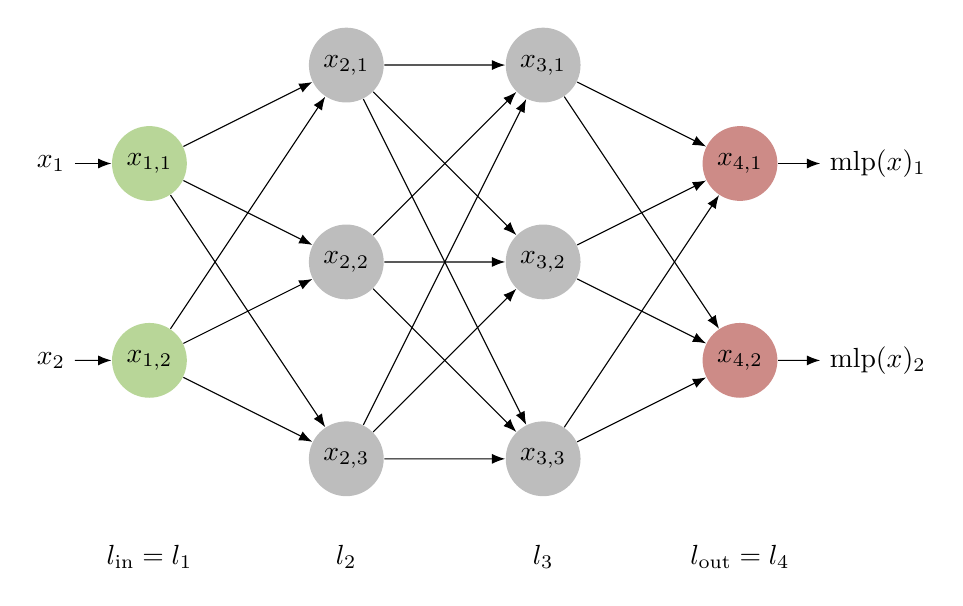
\begin{tikzpicture}[scale = 2.5,
                    neuron/.style={circle}, 
                    input/.style={fill=rwthlightgreen}, 
                    hidden/.style={fill=mgray},
                    output/.style={fill=rwthlightbordeaux}]

    \node[] (nin1) at (-0.5,0) {$x_1$};
    \node[] (nin2) at (-0.5, -1) {$x_2$};
    % input layer
    \node[neuron, input] (n00) at (0,0){$x_{1,1}$};
    \node[neuron, input] (n01) at (0,-1){$x_{1,2}$};
    \node at (0,-2) {$l_\text{in} = l_1$};
    % hidden layer 1
    \node[neuron, hidden] (n10) at (1,0.5){$x_{2,1}$};
    \node[neuron, hidden] (n11) at (1,-0.5){$x_{2,2}$};
    \node[neuron, hidden] (n12) at (1,-1.5){$x_{2,3}$};
    \node at (1,-2) {$l_2$};
    % hidden layer 2
    \node[neuron, hidden] (n20) at (2,0.5){$x_{3,1}$};
    \node[neuron, hidden] (n21) at (2,-0.5){$x_{3,2}$};
    \node[neuron, hidden] (n22) at (2,-1.5){$x_{3,3}$};
    \node at (2,-2) {$l_3$};
    % output layer
    \node[neuron, output] (n30) at (3,0){$x_{4,1}$};
    \node[neuron, output] (n31) at (3,-1){$x_{4,2}$};
    \node at (3,-2) {$l_\text{out} = l_4$};
    
    \node[] (nout1) at (3.7,0) {$\text{mlp}(x)_1$};
    \node[] (nout2) at (3.7,-1) {$\text{mlp}(x)_2$};

    
    % arrows to input
    \draw[-Latex] (nin1) -- (n00);
    \draw[-Latex] (nin2) -- (n01);
    
    % connections input -> hidden 1
    \draw[-Latex] (n00) -- (n10);
    \draw[-Latex] (n00) -- (n11);
    \draw[-Latex] (n00) -- (n12);
    \draw[-Latex] (n01) -- (n10);
    \draw[-Latex] (n01) -- (n11);
    \draw[-Latex] (n01) -- (n12);
    
    % connections hidden 1 -> hidden 2
    \draw[-Latex] (n10) -- (n20);
    \draw[-Latex] (n10) -- (n21);
    \draw[-Latex] (n10) -- (n22);
    \draw[-Latex] (n11) -- (n20);
    \draw[-Latex] (n11) -- (n21);
    \draw[-Latex] (n11) -- (n22);
    \draw[-Latex] (n12) -- (n20);
    \draw[-Latex] (n12) -- (n21);
    \draw[-Latex] (n12) -- (n22);
    
    % connections hidden 2 -> output
    \draw[-Latex] (n20) -- (n30);
    \draw[-Latex] (n20) -- (n31);
    \draw[-Latex] (n21) -- (n30);
    \draw[-Latex] (n21) -- (n31);
    \draw[-Latex] (n22) -- (n30);
    \draw[-Latex] (n22) -- (n31);

    % arrows from output
    \draw[-Latex] (n30) -- (nout1);
    \draw[-Latex] (n31) -- (nout2);
\end{tikzpicture}
            \caption[]{Structure of a fully connected MLP consisting of 4 layers: one input layer (\tikz{\node[circle, fill=rwthlightgreen, minimum size=5pt, inner sep=0pt, outer sep=0pt]{}}), two hidden layers(\tikz{\node[circle, fill=mgray, minimum size=5pt, inner sep=0pt, outer sep=0pt]{}}) and one output layer (\tikz{\node[circle, fill=rwthlightbordeaux, minimum size=5pt, inner sep=0pt, outer sep=0pt]{}}). It computes a function $f:\mathbb{R}^2 \rightarrow \mathbb{R}^2, x = (x_2, x_2) \mapsto \text{mlp}(x)=(\text{mlp}(x)_1,\text{mlp}(x)_2)$}
            \label{fig:mlp}
        \end{figure}
        A multilayer perceptron (MLP) is a type of neural network (NN). An MLP computes a function $f: \mathbb{R}^N \rightarrow \mathbb{R}^M, x \mapsto f(x)$. It can depicted using a number of layers consisting of nodes (see Figure~\ref{fig:mlp}). A multilayer perceptron has $L \geq 3$ layers: one input layer, at least one hidden layer and one output layer.\par
        The input layer $l_{\text{in}}$ consists of $N$ nodes, the output layer $l_{\text{out}}$ consists of $M$ nodes, hidden layers can have an arbitrary number of nodes.\par 
        The $j$-th node in layer $l$ is connected to a value $x_{l,j}$ which is computed from the values of all nodes in the previous layer $l-1$. We define $x_{l_{\text{in}},n} := x_n, n \in [1,...,N]$ and $f(x)_m := x_{l_{\text{out}, m}}, m \in [1,...,M]$. For layers other than the input layer $l-1$ with $I$ nodes and $l$ with $J$ nodes we define $x_{l,j} = h(\sum_{i=1}^{I} x_{l-1,i}\cdot\alpha_{i,j}+\beta_j)$ with an activation function $h$, weights $\alpha_{i,j} \in \mathbb{R}$ and biases $\beta_j \in \mathbb{R}$.
        Weights and biases are trained using error backpropagation. For details on this step we refer to \cite{bishop2006pattern}.
        There are multiple choices for the activation function. For the sake of simplicity, we only consider the rectified linear unit (ReLU) activation function, which is defined as follows:
        \begin{equation*}
            \text{ReLU}(x) \; = \; 
                \begin{cases}
                    x & x \geq 0 \\
                    0 & \text{else}
                \end{cases} \; = \; \text{max}(x,0)
        \end{equation*}
        To be precise, the system described above is a fully connected feed forward neural network. In the following $\text{MLP}(x) := \text{mlp}(x)$ denotes the output of an MLP with input $x$.\par
    \subsection{Satisfiability and Logic}
        In this paper we use logical formulas to formalize the neural network and the function template. While the network can be described through linear constraints, this is not possible for the templates which may have an arbitrary form. Thus, we use quantifier free nonlinear real arithmetic (\texttt{QF\_NRA}). To deal with these formulas, we use an SMT solver. We assume standard settings and notations.
    \section{Approximating an MLP}
\label{sec:mlp}
\begin{figure}
    \centering
        \scalebox{0.75}{
    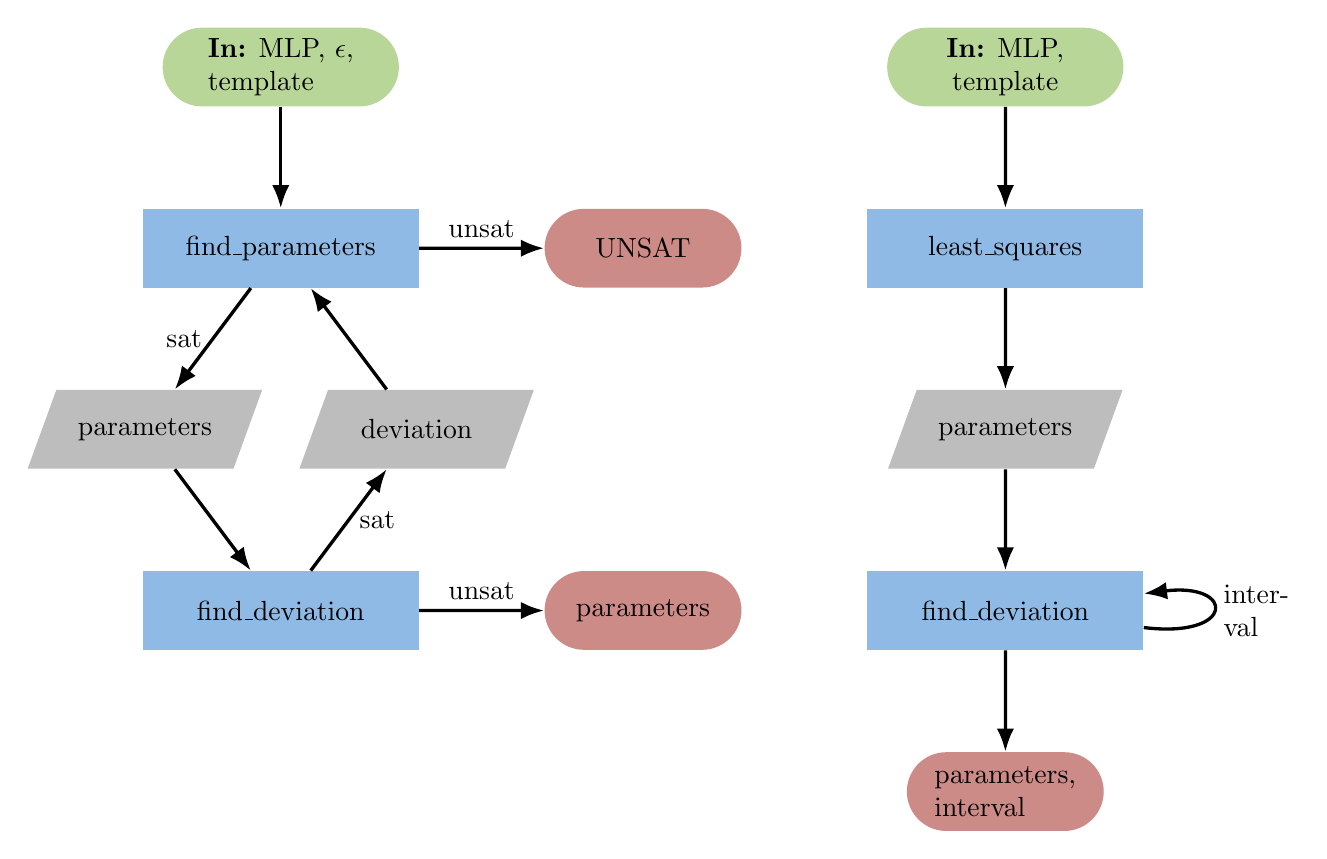
\begin{tikzpicture}[scale = 1.15]
        \coordinate (smt_in) at (0,0);
        \coordinate (smt_find_parameters) at (0, -2);
        \coordinate (smt_find_deviation) at (0, -6);
        \coordinate (smt_unsat) at (4, -2);
        \coordinate (smt_parameters) at (-1.5, -4);
        \coordinate (smt_deviation) at (1.5, -4);
        \coordinate (smt_sat) at (4, -6);
        
        \coordinate (sqr_in) at (8,0);
        \coordinate (sqr_least_squares) at (8, -2);
        \coordinate (sqr_parameters) at (8, -4);
        \coordinate (sqr_find_deviation) at (8, -6);
        \coordinate (sqr_interval) at (8, -8);


        \node[input, align=left] (n_smt_in) at (smt_in) {\textbf{In:} MLP, $\epsilon$,\\ template};
        \node[fproc] (n_smt_find_parameters) at (smt_find_parameters) {\lstinline{find_parameters}};
        \node[fproc] (n_smt_find_deviation) at (smt_find_deviation) {\lstinline{find_deviation}};
        \node[output, align=center] (n_smt_unsat) at (smt_unsat) {UNSAT};
        \node[output, align=left] (n_smt_sat) at (smt_sat) {parameters};
        \node[fio] (n_smt_parameters) at (smt_parameters) {\;\;\;};
        \node[align=left] at (smt_parameters) {parameters};
        \node[fio] (n_smt_deviation) at (smt_deviation) {\;\;\;};
        \node[align=center] at (smt_deviation) {deviation};
    
        \node[input, align=center] (n_sqr_in) at (sqr_in) {\textbf{In:} MLP,\\template};
        \node[fproc] (n_sqr_least_squares) at (sqr_least_squares) {\lstinline{least_squares}};
        \node[fproc] (n_sqr_find_deviation) at (sqr_find_deviation) {\lstinline{find_deviation}};
        \node[output, align=left] (n_sqr_interval) at (sqr_interval) {parameters,\\interval};
        \node[fio] (n_sqr_parameters) at (sqr_parameters) {\;\;\;};
        \node at (sqr_parameters) {parameters};


        \draw[-Latex, very thick] (n_smt_in) -- (n_smt_find_parameters);
        \draw[-Latex, very thick] (n_smt_find_parameters) --node[above]{unsat} (n_smt_unsat);
        \draw[-Latex, very thick] (n_smt_find_parameters) --node[left]{sat} (n_smt_parameters);
        \draw[-Latex, very thick] (n_smt_parameters) -- (n_smt_find_deviation);
        \draw[-Latex, very thick] (n_smt_find_deviation) --node[right]{sat} (n_smt_deviation);
        \draw[-Latex, very thick] (n_smt_find_deviation) --node[above]{unsat} (n_smt_sat);
        \draw[-Latex, very thick] (n_smt_deviation) -- (n_smt_find_parameters);


        \draw[-Latex, very thick] (n_sqr_in) -- (n_sqr_least_squares);
        \draw[-Latex, very thick] (n_sqr_least_squares) -- (n_sqr_parameters);
        \draw[-Latex, very thick] (n_sqr_parameters) -- (n_sqr_find_deviation);
        \draw[-Latex, very thick] (n_sqr_find_deviation) -- (n_sqr_interval);
        \draw[-Latex, very thick] (n_sqr_find_deviation) edge[loop]node[right, align=left]{inter-\\val} (n_sqr_find_deviation);
    \end{tikzpicture}
}
    \caption[]{High-level flow-chart diagram for Algorithms \ref{lst:smt_default}, \ref{lst:smt_optimize} (left) and~\ref{lst:fit_verify}~(right) using Algorithm~\ref{lst:nn_verify}.}
    \label{fig:alg}
\end{figure}
In this section we give a detailed description of the algorithms we implemented. A high-level flow-chart diagram of the algorithms can be found in Figure~\ref{fig:alg}.


\subsection{Finding deviations}
    \label{subsec:nn_verify}
    \begin{tcolorbox}[arc=0mm, colback=rwthlightgray, outer arc=0mm, colframe = white, size=small, bottom=-9mm]
        \begin{lstlisting}[caption={Method to find a deviation between the function and the MLP}, label=lst:nn_verify, mathescape=true]
def find_deviation(template, parameters, MLP, 
                   ub, lb):
    
    # insert parameters in template to define f
    f = template(parameters)
	
    # encode conditions
    encoding = $\exists x: |\text{MLP}(x)-\text{f}(x)| > \epsilon \land (\text{lb} \leq x \leq \text{ub})$
    
    # use an external solver to find a solution
    Solver.add(encoding)
    result = Solver.check()
    
    if result == SAT:
        model = Solver.model()
        return model($x$)
    return UNSAT
\end{lstlisting}
    \end{tcolorbox}
    \vspace{9mm}
    All of the approaches we propose rely on the \lstinline{find_deviation} method, which verifies whether found parameters for the function template yield a function that approximates the behaviour of the given MLP on a specified interval within some error bound $\epsilon$. For this we encode the input-output relation of the MLP as introduced in \cite{DBLP:journals/corr/abs-2008-01204}. Pseudocode of the presented algorithm can be found in Algorithm~\ref{lst:nn_verify}.\par
    We construct a formula encoding the existence of values for the variables $x$ and $y$ such that $\text{MLP}(x)=y$. Accordingly, we encode the existence of values for the variables $x'$ and $y'$ such that $f(x')=y'$. Be $lb$ a lower bound and $ub$ an upper bound defining an input subspace. We assert both the encoding of the MLP and the function, with the found parameters to an of-the-shelf SMT-solver and further encode
    \begin{align*}
    	x = x' \land x \geq lb \land x \leq ub \\
    	y - y' > \epsilon \lor y' - y > \epsilon
    \end{align*}
    The concatenation of these formulas is satisfiable if and only if there is some input in the specified subspace such that the output of $f$ and the MLP deviate more than $\epsilon$.
    The model returned by the solver provides this input value.\par
    To improve the solving time we developed a strategy to split the encoding of this problem into smaller sub-problems, which then can be solved in parallel. This is accomplished by omitting the encoding of the behaviour of the activation function ReLU for a node and instead solving two formulas, where the input of the node is limited such that the output of the node is linear to the input. We refer to this as a \textit{split}.

\subsection{SMT-based Parameter Search}
    \label{subsec:smt}
    In this section, we describe two SMT-based variants for finding parameters of the given template. The left side of Figure~\ref{fig:alg} is an abstraction which works for both variants. The two variants differ in their realization of the \lstinline{find_parameters} method.
    \subsubsection{Template Adjustment within $\epsilon$}
    \label{subsubsec:smt1}
        \begin{tcolorbox}[arc=0mm, colback=rwthlightgray, outer arc=0mm, colframe = white, size=small, bottom=-9mm]
            \begin{lstlisting}[caption={Finding parameters within $\epsilon$.}, label=lst:smt_default, mathescape=true]
def find_parameters(template, MLP, $\epsilon$, x):

    # encode conditions
    encoding = $ ( \exists \text{parameters}: f = \text{template(parameters)}$
                $\land \ |f(x) - \text{mlp}(x)| \leq \epsilon )$

    # use an external solver to find a solution
    Solver.add(encoding)
    result = Solver.check()

    if result == SAT:
        model = Solver.model()
        return model(parameters)
    return UNSAT
\end{lstlisting}
        \end{tcolorbox}
        \vspace{9mm}
        Our fist approach consists of the routine summarized in Algorithm~\ref{lst:smt_default}.
        The input to our algorithm consists of a function template, an MLP, a maximal deviation $\epsilon$ and an lower and upper bound for the input $lb, ub$. We start by encoding the output $y$ of the template function for some arbitrary, fixed input (e.g. $x=lb$) in dependence of the parameters and add the requirement that $y-\text{mlp}(x) \leq \epsilon \land \text{mlp}(x)-y \leq \epsilon$. Note that here $\text{mlp}(x)$ and $x$ are constant values and $\epsilon$ is part of the input. The resulting formula has a model if and only if the there are parameters for the template such that the resulting function deviates at most $\epsilon$ from the MLP.\par
        In the second step we call the \lstinline{find_deviation} method to determine whether the found parameters are within the $\epsilon$ error bound for the entire subspace. If this is the the case, the method terminates. Otherwise the we use the counterexample provided by \lstinline{find_deviation} to repeat the first step.\par
        During the process the first step will be repeated for different inputs. For efficiency we use an incremental solver and assert the encoding for a different input in each iteration on top of the previous formulas. This way the resulting parameters satisfy the requirement of the maximal deviation for the entire set of input samples.
        
    \subsubsection{Template Adjustment with Optimal $\epsilon$}
    \label{subsubsec:smt2}
        \begin{tcolorbox}[arc=0mm, colback=rwthlightgray, outer arc=0mm, colframe = white, size=small, bottom=-9mm]
            \begin{lstlisting}[caption={Finding parameters minimizing $\epsilon_{\text{max}}$.}, label=lst:smt_optimize, mathescape=true]
def find_parameters(template, MLP, X):

    # encode conditions
    encoding = $\big( \; \exists \, \text{parameters}, \epsilon_{\text{max}}:$
                $ f = \text{template(parameters)}$
                $\bigwedge_{x \in X} \ |f(x) - \text{mlp}(x)| \leq \epsilon_{\text{max}}$
                $\land \ (\bigvee_{x \in X} \ |f(x) - \text{mlp}(x)| = \epsilon_{\text{max}}) \; \big)$

    # use an external solver to find a minimal 
    # solution
    Solver.add(encoding)
    result = Solver.minimize($\epsilon_{\text{max}}$)

    if result == SAT:
        model = Solver.model()
        return model(parameters)
    return UNSAT
\end{lstlisting}
        \end{tcolorbox}
        \vspace{9mm}
        The approach described in this section is summarized in Algorithm~\ref{lst:smt_optimize}. If we only consider function templates, which can be encoded using linear real arithmetic, we can use existing solvers \cite{DBLP:conf/tacas/BjornerPF15} to find the minimal $\epsilon$ and parameters for the template such that for the resulting function $f$ it holds that for all $x \leq ub, x \geq lb$, $|f(x) - \text{mlp}(x)| \leq \epsilon$.\par
        This can be accomplished by modifying the first step of the previously introduced approach.
        Be $X= \{x_0, ..., x_{k-1} \}$ the set of input values in the k-th iteration.
        In stead of encoding the requirement $y_i-\text{mlp}(x_i) \leq \epsilon\; \land\; \text{mlp}(x_i)-y_i \leq \epsilon$ for all $x_i \in X$,
        we encode for each $x_i \in X$ the deviation of the MLP output and the function:
        \begin{align*}
            (y_i - \text{mlp}(x_i) \geq 0) &\rightarrow (e_i = y_i - \text{mlp}(x_i) )\; \land \\
            (\text{mlp}(x_i) - y_i > 0) &\rightarrow (e_i = \text{mlp}(x_i) - y_i)
        \end{align*}
        With that we can encode the maximal deviation:
        \begin{align*}
            \bigvee_{x_i \in X} ( \epsilon_{\text{max}} = e_i )\; \land \\
            \bigwedge_{x_i \in X} ( \epsilon_{\text{max}} \geq e_i)
        \end{align*}
        Finally, let the solver find a model of the encoding with the target function of minimizing $\epsilon_{\text{max}}$.


    \subsection{Least-Squares Fit}
        \label{subsec:sqa}
        \vspace{0.3cm}
        \begin{tcolorbox}[arc=0mm, colback=rwthlightgray, outer arc=0mm,colframe = white, size=small, bottom=-9mm]
            \begin{lstlisting}[caption={Method to fit parameters and find a deviation interval}, label=lst:fit_verify, mathescape=true]
def fit_verify(mlp_model, target_function, interval, 
               size, epsilon, accuracy_steps):

    # take samples
    x, mlp(x) = sample(mlp_model, interval, size)

    # find parameters of target function
    parameters = least_squares(x, mlp(x), 
                               target_function)

    # binary search to narrow down deviation 
    # interval
    lower = 0
    upper = epsilon
    for _ in range(accuracy_steps)
        mid = (lower + upper)/2
        if find_deviation(mid):
            lower = mid
        else:
            upper = mid
    deviation_interval = [lower, upper]

    return parameters, deviation_interval
\end{lstlisting}
        \end{tcolorbox}
        \vspace{9mm}
        Another approach we tested is using existing, traditional least-squares fit. Pseudo-code of the the method can be found in Algorithm~\ref{lst:fit_verify}, the right side of Figure~\ref{fig:alg} shows a high-level flow-chart diagram of the approach.\par
        We used existing implementations of linear regression for linear functions of arbitrary dimension and polynomial fitting for 1D polynomials of arbitrary degree. Details on the functions used are in Section~\ref{sec:imp}.\par
        These methods take a number of $(x,f(x))$ pairs and then find the parameters for the best fitting curve. Thus, we take input/output samples of the neural network. The current implementation takes evenly spaced samples in a specified interval.\par
        In contrast to the SMT methods from Section~\ref{subsec:smt}, we are not able to enforce the parameters to fulfill certain properties. Therefore, we are not able to use $x$ values with large deviation to refine the parameters. We are only able to check whether there exists a value $x$ a with minimum deviation $\epsilon$, meaning ${\text{mlp}(x)-f(x)\leq\epsilon}$. Therefore we use binary search to find an interval that is guaranteed to contain the maximal distance between the curve found and the output of the MLP. Since MLPs using only ReLU activation functions are picewise linear, it would also be possible to find the maximum deviation analytically. This could be part of further research.\par
        %\paragraph{Correctness}
        %In the first part of the algorithm we use existing least-squares implementations and rely on their correctness. As binary search is a well-known and widely-used concept in computer science we omit a proof of correctness in this paper. A proof for soundness and completeness of \lstinline{find_deviation} can be found in Section~\ref{subsec:nn_verify}. 
    \section{Implementation}
\label{sec:imp}
    The implementation can be found in our GitHub repository \cite{Dirks_mlp_smt_closed}.  We used the language Python for the implementation.\par %TODO: reference documentation if running
    To create, train and store MLPs, we used \lstinline{tensorflow} with \lstinline{keras} and \lstinline{sklearn}. For solving the formulas we used \lstinline{z3}. \par
    For curve fitting we used existing least-squares fit implementations. For linear regression we used \lstinline{sklearn.linear_model.LinearRegression}, for polynomial fitting \lstinline{numpy.polynomial.polynomial.polyfit}.
    \section{Evaluation}
    \label{sec:eva}
    \begin{table}
        \centering
        \begin{tabular}{|p{2cm}|p{4cm}|p{4cm}|}
            \hline
                            & SMT                                       & Least-Squares Curve Fitting \\
            \hline
            \hline
            similarities    & \multicolumn{2}{p{8cm}|}{\tabitem tries to find a curve fitting to the MLP} \\
                            & \multicolumn{2}{p{8cm}|}{\tabitem uses an SMT solver to check whether parameters fulfil given bounds} \\
            \hline
            differences     & \tabitem \textit{incrementally} includes outliers to find parameters   
                                                                        & \tabitem uses existing methods \textit{once} to find parameters
            \\              & \tabitem indirectly considers all points when finding new parameters
                                                                        & \tabitem only considers a finite set of points to find parameters
            \\
                            & \tabitem can guarantee that parameters with certain accuracy do not exist
                                                                        & \tabitem can only give guarantee for the accuracy of parameters found by the fitting function
            \\
                            &                                           & \tabitem incapable of improving parameters\tablefootnote{It may be possible to improve the parameters through modifying meta-parameters of the fitting function, e.g. the number of samples. However, this does not guarantee improvement. Also including an outlier in the fitting process does not give any guarantees w.r.t. accuracy.}\\
            \hline
        \end{tabular}
        \caption{Methodical comparison of the SMT approach and existing curve fitting approaches.}
        \label{tab:com}
    \end{table}.
    Due to the novelty of this approach (see Section~\ref{sec:rel}), it is impossible for us to compare it to existing ones. Due to the methodical differences of the presented approaches (see Table~\ref{tab:com}), comparing them quantitatively with each other is also not sensible. Therefore we can (1) qualitatively evaluate the approaches and (2) quantitatively evaluate the approaches through comparing the performance of the same approach on different MLPs.\par
    A methodical comparison can be found in Table~\ref{tab:com}.\par
    \begin{table}[h]
        \centering
            \begin{tabular}{|l|r|r|r|r|}
                 \hline
                 Template &  \#Nodes    & $\epsilon$ & \#Splits     & Runtime in \si{\s}\\
                 \hline
                 \hline
                 1D linear function        &    12             & 0,5         & 0& 1,23\\
                                           &                   &           & 1& 4,18\\ \hline
                 2D linear function        &    14             & 0,5         & 0& -\\
                                           &                   &           & 1& 6174.98\\ \hline
                 1D polynomial             &    12             & 0,5         & 0& 8,10 \\
                 of degree 2               &                   &           & 1& 7,44\\ \hline
                 1D polynomial             &    17             & 0,5         & 0& 6.34\\
                 of degree 3               &                   &           & 1& 6.87\\ \hline
                 1D linear function        &    57             & 0,5         & 0& -\\
                                           &                   &           & 1& -\\ \hline
            \end{tabular}
        \caption{Test results for the method described in section \ref{subsubsec:smt1}. A timeout is denoted with -.}
        \label{tab:smt_default}
    \end{table}
    \begin{table}
        \centering
            \begin{tabular}{|l|r|r|r|r|}
                 \hline
                 Template &  \#Nodes    & $\epsilon$ & \#Splits     & Runtime in \si{\s}\\
                 \hline
                 \hline
                 1D linear function        &    12             & 0,02         & 0& 4,38\\
                                           &                   &              & 1& 5,87\\ \hline
                 2D linear function        &    14             &           & 0& -\\
                                           &                   &           & 1& -\\ \hline
                 1D linear function        &    57             &             & 0& -\\
                                           &                   &           & 1& -\\ \hline
                 
            \end{tabular}
        \caption{Test results for the method described in section \ref{subsubsec:smt2}. A timeout is denoted with -. The found bounds for $\epsilon$ are rounded to two decimal places.}
        \label{tab:smt_optimize}
    \end{table}
    \begin{table}
        \centering
            \begin{tabular}{|l|r|r|r|r|}
                 \hline
                 Template &  \#Nodes    & $\epsilon$ & \#Splits     & Runtime in \si{\s}\\
                 \hline
                 \hline
                 1D linear function        &    12             & [0,02; 0,03] & 0& 3,07\\
                                           &                   &           & 1& 5,25\\ \hline
                 2D linear function        &    14             & [0,08; 0,09] & 0& 36,90 \\
                                           &                   &           & 1& 30,57 \\ \hline
                 1D polynomial             &    12             & [0,31; 0,33] & 0& 1,47 \\
                 of degree 2               &                   &           & 1& 3,53\\ \hline
                 1D polynomial             &    17             & [0,25; 0,27] & 0& 1,63 \\
                 of degree 3               &                   &           & 1& 3,80\\ \hline
                 1D linear function        &    57             &             & 0& -\\
                                           &                   &           & 1& -\\ \hline
            \end{tabular}
        \caption{Test results for the method described in section \ref{subsec:sqa}. A timeout is denoted with -.}
        \label{tab:least_squares}
    \end{table}
    All tests were executed on the Intel Xeon Platinum 8160 Processors “SkyLake” (2.1 GHz) with 8 GB of memory. Each test with zero splits was given one CPU core and each test with one split was given two CPU cores and a timeout of 5 hours. Only the tests for the MLP with 57 nodes were given 16 GB of memory.\par
    Table~\ref{tab:smt_default} and~\ref{tab:smt_optimize} show runtimes of the methods described in Section~\ref{subsubsec:smt1} and~\ref{subsubsec:smt2}, respectively. The number of timeouts show that optimizing the parameters w.r.t. $\epsilon$ did not improve the runtime and lead to a notable number of timeouts. Splitting at certain nodes for parallelization did also not improve runtime.
    Table~\ref{tab:least_squares} shows the results of the method described in Section~\ref{subsec:sqa}. We can see that this approach worked quite well and was also able to give relatively small deviation intervals using only 4 interval-refinement steps. However, \lstinline{find_deviation} repeatedly lead to a timeout on a network with 57 nodes.\par
    We can generally observe that larger models lead to timeouts. Although repeatedly tried, we were not able to get results for any model with more than 20 nodes.
    \section{Related Work}
    \label{sec:rel}
    To the best of our knowledge, extracting function from a trained MLP has not been investigated. However, part of our approach is MLP formalization and the verification of its properties (for details see Section~\ref{subsec:nn_verify}). Neural network verification is a big field of study and there exists an abundance of approaches we could have used or adapted for our own implementation. It should be mentioned that the problem of network verification is mostly not interpreted as proving a direct functional relation between input and output. Thus, if an existing approaches is used for our task, we would most likely have to adapt it. For an in depth overview of verification algorithms for neural networks we refer to \cite{liu2019algorithms}. As performance was not a main priority, we omitted related work and did our own straight forward encoding and solving using \lstinline{z3} as described in Section~\ref{sec:imp}. Future work with focus on performance could use existing, more sophisticated approaches.

\begin{comment}
    A selection of some well know approaches is listed below. 
    %Very small portion of the related work existing w.r.t. the "verification part"
    %(background: a big field of study focuses on verifying certain "good" properties/specifications that NNs should have, often to prove the absence of adversary examples/ close miss-classifications => formalization of the NN (e.g. through z3), but not necessarily "general/functional" input-output relations)\par
    %todo: beatify list, sentences ...
    \paragraph{}
    \begin{itemize}
        \item A Unified View of Piecewise Linear Neural Network Verification
            \begin{itemize}
            	\item https://arxiv.org/pdf/1711.00455.pdf
            	\item model function as part of network then check whether >/=/< 0.
            	\item only linear dependencies of input/output        
        	\end{itemize}
        \item Reluplex: An Efficient SMT Solver for Verifying Deep Neural Networks
            \begin{itemize}
            	\item https://arxiv.org/abs/1702.01135
            	\item fast modelling of NNs with ReLU functions (fancy techniques)
            	\item input [a,b] -> output [c,d] ?        
        	\end{itemize}
        \item Verification of a Trained Neural Network Accuracy (old paper)
            \begin{itemize}
                \item https://ieeexplore.ieee.org/document/938410 (maybe first time that some kind of verification was applied???)
                \item error bounds in comparison to lookup table for input intervals
                \item grid, bound on growth rates between grid points
            \end{itemize}
        \item Challenging SMT solvers to verify neuralnetworks
            \begin{itemize}
            	\item https://dl.acm.org/doi/10.5555/2350156.2350160
            	\item formalize NN in logic to prove the following properties
    		    \begin{itemize}
    		        \item stability
            		\item local safety 
            		\item global safety        
    		    \end{itemize}
    	    \end{itemize}
        \item Safety verification of deep neural networks (very often cited!)
            \begin{itemize}
            	\item https://link.springer.com/chapter/10.1007/978-3-319-63387-9\_1
            	\item proof existance of "no-change-of-class" region around all points-> absence of weird behaviour
        	\end{itemize}
        \item Verification of Non-Linear Specifications for Neural Networks
            \begin{itemize}
                \item https://arxiv.org/abs/1902.09592
            	\item incomplete method to verify non-linear properties
            \end{itemize}
        \item NNV tool (Abrahams tip)
        \item NNENUM - Stanley Bak:

nnenum: Verification of ReLU Neural Networks with Optimized Abstraction Refinement. NFM 2021: 19-36
        \end{itemize}
\end{comment}
    
    \section{Conclusion \& Outlook}
\label{sec:con}
We presented approaches for finding a closed form of MLPs which combined relatively simple ideas and existing methods.\par
%theoretical consequences of fixes
The first approach described in Section~\ref{subsec:smt} used a counterexample-guided search algorithm for parameters using a type of NN-verification. The evaluation showed that this approach does work in practice, however, scalability to larger networks or more complex functions is still an issue. Future work could try different methods to scale the approach to more realistic network sizes. Another topic of interest could be to directly optimize the parameters w.r.t. the maximum deviation and not their sum.\par % try to optimize w.r.t. max deviation in first place
%completeness???
Reusing the NN-verification of the first approach, the second approach used existing least-squares implementations to find parameters. Of course, finding parameters initially is much faster process. However, the least-squares the optimization considers only a finite set of points and optimizes w.r.t. least squares and therefore solves a different problem. As the function \lstinline{find_deviation} was used in this approach as well, scalability issues were apparent too.\par
Another possible topic for future work, which would affect both approaches, could be to rewrite the function \lstinline{find_deviation} so that it returns the maximum difference between the MLP and the function found. However, being an optimization problem, the runtime of this alternative implementation would be even longer.\par
In conclusion, we were able to present usable approaches for finding a closed form of MLPs. To be usable for real-world applications, future work is necessary.
    \printbibliography
\end{document}